%---------------- COMMENT FOR IMPORTING ----------------------
%\RequirePackage{lineno}					%Comment for importing
%\documentclass[12pt]{report}		%Comment for importing
%\pagestyle{headings}
%\input{ST-input2}								%Comment for importing

%\setcounter{chapter}{2}
%\begin{document}								%Comment for importing
%\setpagewiselinenumbers
%\linenumbers
%\tableofcontents
\graphicspath{{Chapter3/figures/}} 

%-------------------------------------------------------------

\chapter{Application: Clustering Insurance Data}
\label{chap:datasets}
%\begin{itemize}
%\item Chunking
%\item Simple clustering
%\item Similarity metrics
%\item Small study of variation of quotes
%\item How useful is a Clusteram summary for simple analystics (population comparions/t-tests)
%\item How is this effected by nMicro and weighting?
%\item How representative are the microclusters? Outliers? Confidence?
%\end{itemize}

A car insurance company offers an online quote service. The customer enters certain details above themselves and their car, and they recieve 3 quotes relating to the three types of policies offered. The data consists of 465115 requests for car insurance quotes collected online continuously over a period of three months. The aim is to perform initial analysis of the data set, explore more to understand and learn about the customer base. We will also look at performing clustering algorithms on the data, treating it both as a large offline data set and as an evolving data stream. 

\section{Data Exploration}
 
This section will describe the data and relevant characteristics of the variables. The customer features are Age of Driver, Age of Car, Expected Value of Car, CC and policy duration. The three Value features are outcomes relating to the customer features and such should be treated differently. There are eight features which we will split into five customer features and three quote features. The quote features are outcomes depending on the customer features and such should be treated separately. We will consider the customer features first.

\subsection{Customer Features}
\label{customer-features}

There are five customer features available in the data set. Four of these are interval variables, and duration one is a symmetric binary variable. Standard statistical summaries for the four interval variables are shown in Table \ref{tab:cf_summaries}.

\begin{table}[h]
\begin{center}
 \begin{tabular}{lrrrrrrr}
& Min & Max & Mean & Std Dev & Median &
Skewness & Kurtosis \\
\hline
Age of Driver & 18 & 81 & 46.03 & 13.00 & 44 & 0.52 & 2.57 \\
Age of Car & 0 & 31 & 10.90 & 5.25 & 11 & 0.40 & 3.25 \\
Expected Value of Car & 1000 & 99999 & 5319.51 & 4967.40 & 4000 & 3.60 & 38.23 \\
CC & 100 & 7000 & 1445.80 & 325.23 & 1390 & 2.40 & 20.86\\
\end{tabular}
\caption{Statistical summaries for customer features}
\label{tab:cf_summaries}
\end{center}
\end{table}

Skewness is a measure of symmetry, or more precisely, the lack of symmetry. A distribution, or data set, is symmetric if it looks the same to the left and right of the center point.

Kurtosis is a measure of whether the data are heavy-tailed or light-tailed relative to a normal distribution. That is, data sets with high kurtosis tend to have heavy tails, or outliers. Data sets with low kurtosis tend to have light tails, or lack of outliers. 

Figure \ref{fig:boxplots_cf} shows the boxplots for four customer variables, allowing us to observe  the skewness and outliers in each feature.

\begin{figure}[H]

\begin{subfigure}{.24\textwidth}
  \centering
  \includegraphics[width=\linewidth]{exploration_files/figure-latex/dist_boxplots-1.pdf}
  \caption{Age of Driver}
\end{subfigure}
\begin{subfigure}{.24\textwidth}
  \centering
  \includegraphics[width=\linewidth]{exploration_files/figure-latex/dist_boxplots-2.pdf}
  \caption{Age of Car}
\end{subfigure}
\begin{subfigure}{.24\textwidth}
  \centering
  \includegraphics[width=\linewidth]{exploration_files/figure-latex/dist_boxplots-3.pdf}
  \caption{Expected Value of Car}
\end{subfigure}
\begin{subfigure}{.24\textwidth}
  \centering
  \includegraphics[width=\linewidth]{exploration_files/figure-latex/dist_boxplots-4.pdf}
  \caption{CC}
\end{subfigure}
\caption{Boxplots for the Customer Features}
\label{fig:boxplots_cf}
\end{figure}

We see that all four variables have some positive skew, this is particularly noticiable for the Expected Value of Car and CC. The presence of outlier is also evident in Expected Value and CC, with Expected Value in particular having a very long tail due to the dominating outliers. 


The final customer feature is the policy duration. The customer can select if they are interested in a 6 or 12 month policy. Policy duration
takes only two values, 6 months or 12 months. We shall treat this as a symmetric binary variable ``isthepolicy6months''. There are roughly an
equal amount of both types of policies. In the data set there are 224578 6 months policies and 240537 12 month policies.

\subsection{Quote features}
\label{quote-features}

The data also consists of three features, Value A, Value B and Value C. These are policy prices offered to the customer given their input. The
summary statistics for there features are given in Table \ref{tab:value_summaries}.


\begin{table}[h]
\begin{center}
 \begin{tabular}{lrrrrrrr}
& Min & Max & Mean & Std Dev & Median &
Skewness & Kurtosis \\
\hline
Value A & 44 & 701 & 173.67 & 65.13 & 167 & 0.66 & 3.21\\
Value B & 56 & 716 & 192.28 & 69.52 & 188 & 0.53 & 2.75\\
Value C & 75 & 1667 & 231.27 & 85.16 & 225 & 0.63 & 3.58\\
\end{tabular}
\caption{Statistical summaries for the quotes}
\label{tab:value_summaries}
\end{center}
\end{table}

Value A $<$ Value B $<$ Value C is always true for each row, therefore I assume that Value A is a basic policy, and Value C is a
premium policy. We can also look at a plot of the sorted Values to see how they interact.

\begin{figure}[h]
  \centering
 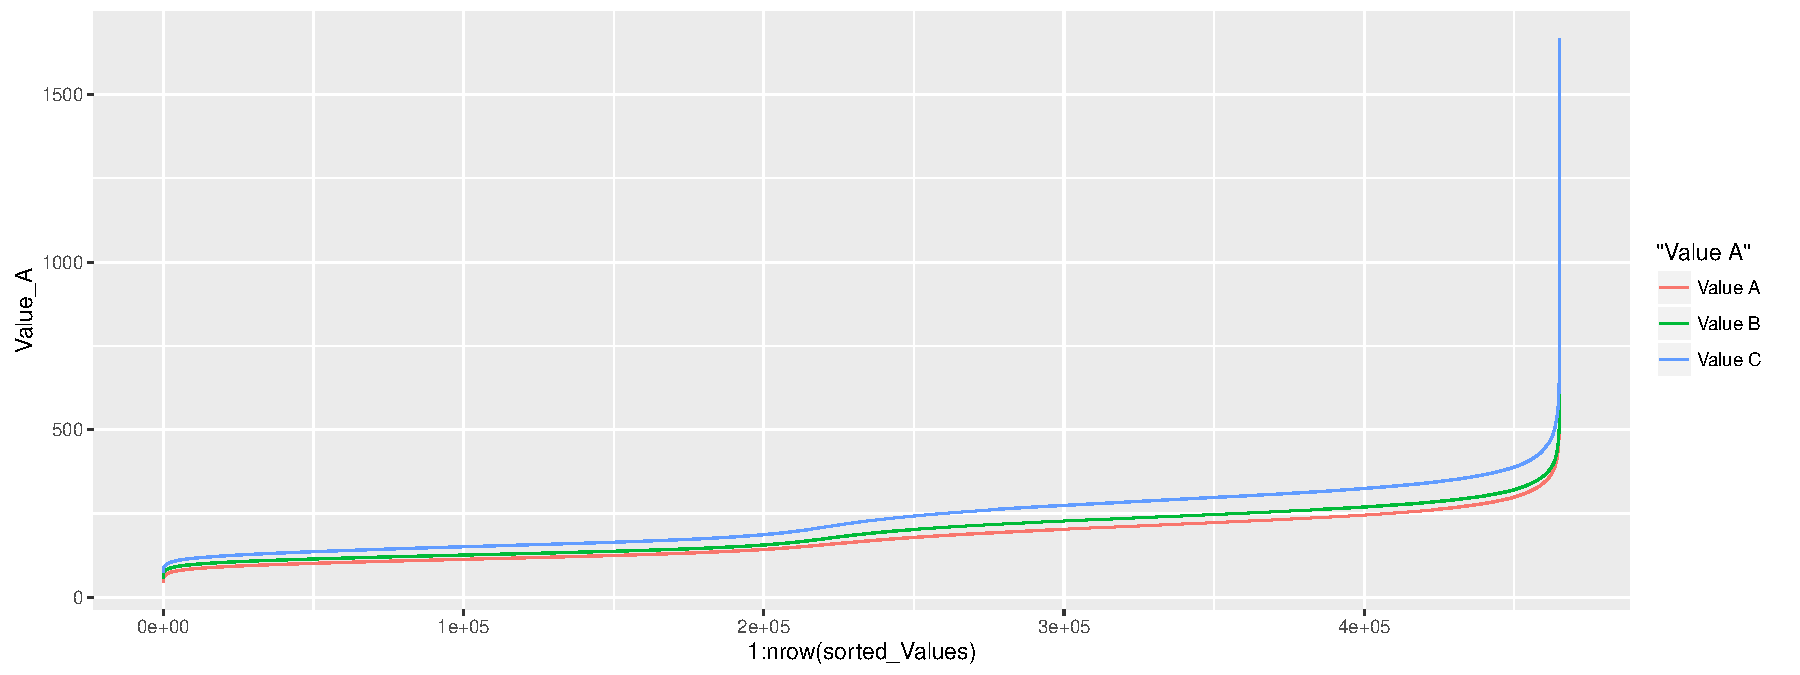
\includegraphics[width = 10cm]{exploration_files/figure-latex/values_sorted-1.pdf} 
  \caption{Quotes}
\end{figure}

There is a clear relationship between the three quotes offered. I will consider only the standard policy (Value B) in further analysis.

\subsection{Correlation between variable}

Correlation between variables can cause problems for regression because of multicollinearity. Also, it can indicate that some variables are redundant. For interval variables matrix scatterplots were used. From these, the only strong correlation indicated was between MORTDUE and VALUE.



correlation (scatter plots, chi squared)


\subsection{Stream velocity}
\label{streaming-aspect}

As stated above, the data is recieved as a stream, and thus we have timestamped data. It is worth examining how the volume of data evolves
over the stream. We have approximately 3 months of data. 

\begin{figure}[h]
  \centering
  \includegraphics[width = 10cm]{exploration_files/figure-latex/observations_per_day-1.pdf}
  \caption{Volume of calls per day}
\label{fig:calls_per_day}
\end{figure}


We can see in Figure \ref{fig:calls_per_day} that more requests are recieved on week days than on weekends as might be expected. We can also observe the 

\begin{figure}[h]
  \centering
\includegraphics{exploration_files/figure-latex/distribution_of_requests-1.pdf}  
  \caption{Peak quote request times}
\label{fig:peak_times}
\end{figure}

Figure \ref{fig:peak_times} shows the distribution of requests over time of day. This  is what we would expect to see with peak number of requests occuring beteen 10am and 7pm.

% Finally we can look if there exists any sort of seasonal trend within the volume of calls, as seen in Figure \ref{fig:seasonal}.
% \begin{figure}[h]
%   \centering
% \includegraphics{exploration_files/figure-latex/total_requests_policy_duration_week-1.pdf}  
%   \caption{Seasonal }
%   \label{fig:seasonal}
% \end{figure}

\section{Pre-processing}
%\input{Chapter3/}t
Transform variables so that the variables are approximately normal. Check skewness, kurtosis, QQ plot, boxplot.

For simplicity we only consider the 12 month policy quotes. There are 240537 quotes. 
We exclude any very expensive cars nd high engine cars from the analysis data set. This is because they might be outliers, there are some very suspicious values. Also removing these points allows us to visualise the rest of the data more easily. 
We exclude all cars with a value $>$ \pounds30,000 or with an engine size $>$ 4000cc. This removes 1056 datapoints, only 0.5\% of the data. 

We can visualise the correlations of the remaining variable as in Figure \ref{fig:ggpairs_corr}.

\begin{figure}[!h]
  \centering
  \includegraphics[width = 16cm, height = 16cm]{ggpairs_valueB_sample_5000.pdf}
  \caption{Pairwise correlation and density plots}
  \label{fig:ggpairs_corr}
\end{figure}

We can see that the two most negatively correlated features are Expected Value of Car and Age of Car. This makes sense as we expect older cars to be worth less. There is also some correlation evident between the Value of the Car and the Engine size. We would expect that cars with bigger engines may be more expensive. This correlation is not as strong as that between car value and age of car.



\section{Regression}

  Read in raw data.
  Consider only 12 month policies.
  Exclude any expensive cars (\textgreater{} £30,000)
  Exclude any cars with engine size \textgreater{} 4L

We exclude any very expensive cars and high engine cars from the data
set. This is because they might be outliers (some very suspicious
values). Also removing these points allows us to visualise the rest of
the data more easily. By excluding all cars \textgreater{} £30,000 or
with an engine size \textgreater{} 4000, we remove 1056 quotes
(\textasciitilde{}0.5\% of the 12 month quotes.)

Transformations

We apply a log transform to the Expected Value. Clustream streaming
seems to been having issues with Expected Value of Car unless I
transform it with log or sqrt or similar.

\includegraphics{offline_regression_files/figure-latex/fighold-1.pdf}
\includegraphics{offline_regression_files/figure-latex/fighold-2.pdf}

Regression on the full dataset

The R function step() can be used to perform variable selection. To
perform forward selection we need to begin by specifying a starting
model and the range of models which we want to examine in the search.

We can perform forward selection. This tells R to start with the null
model and search through models lying in the range between the null and
full model using the forward selection algorithm. It gives rise to the
following output:

This indicates that we should use all possible predictors in our linear
model.


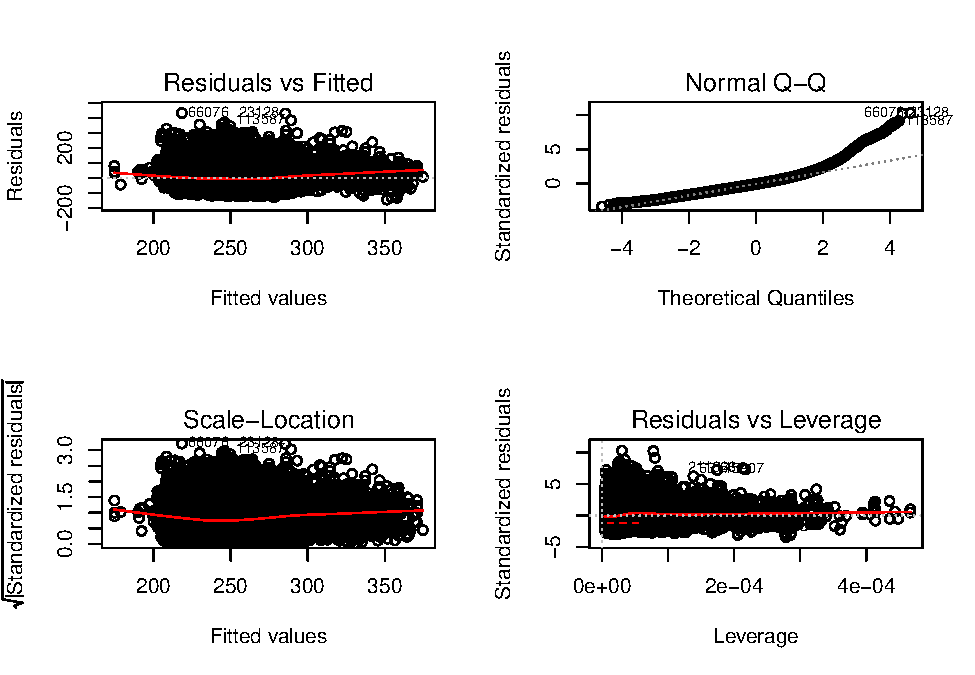
\includegraphics{offline_regression_files/figure-latex/unnamed-chunk-4-1.pdf}

We can also view the actual against predicted.


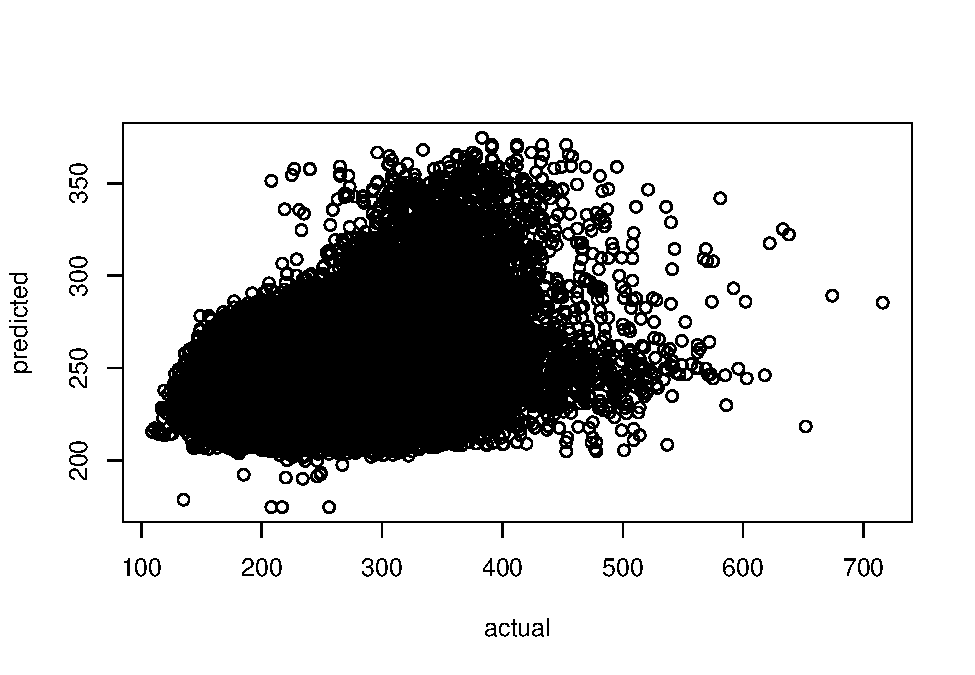
\includegraphics{offline_regression_files/figure-latex/unnamed-chunk-5-1.pdf}


Online Regression

  Treat the dataset as a datastream
  Initialise the clustream algorithm with 1000 data points.
  Increment the data stream by 2000 points, tracking with Clustream
  Use the clustream microcluster centers as input to a linear model
  (same set up as offline)
  Store the coefficients from the model
  Repeat the last 3 steps until the end of the stream


This procedure is carried it with the following three algorithms;
Clustream, weighted Clustream and a windowed approach.

We vary the nMicro clusters / window size used.

Using this we can plot how the coeffients change each time a linear
model is created.

\includegraphics{offline_regression_files/figure-latex/unnamed-chunk-6-1.pdf}

We can view how the coeffcients for all of the model predictors change
over time for different algorithms as shown in the plot above. However
this is messy to look at, and viewing the results for varying number of
microclusters would make things even more confusing.

Instead we focus on the absolute mean error from the coefficient given
in the offline model, and the variance of the coefficients.

Mean Abs Error Plots

\includegraphics{offline_regression_files/figure-latex/unnamed-chunk-7-1.pdf}
\includegraphics{offline_regression_files/figure-latex/unnamed-chunk-7-2.pdf}
\includegraphics{offline_regression_files/figure-latex/unnamed-chunk-7-3.pdf}
\includegraphics{offline_regression_files/figure-latex/unnamed-chunk-7-4.pdf}
\includegraphics{offline_regression_files/figure-latex/unnamed-chunk-7-5.pdf}

Variance Plots

\includegraphics{offline_regression_files/figure-latex/unnamed-chunk-8-1.pdf}
\includegraphics{offline_regression_files/figure-latex/unnamed-chunk-8-2.pdf}
\includegraphics{offline_regression_files/figure-latex/unnamed-chunk-8-3.pdf}
\includegraphics{offline_regression_files/figure-latex/unnamed-chunk-8-4.pdf}
\includegraphics{offline_regression_files/figure-latex/unnamed-chunk-8-5.pdf}



\section{Clustering offline}

\section{Dataset 2}

3210515 x 29. brand - anytime or Interamerica. 
Duration of call - type of policy/brand/gender?

%---------------- COMMENT FOR IMPORTING ----------------------
%\pagebreak											%Comment for importing
%\bibliographystyle{plainnat}		%Comment for importing
%\bibliography{References}				%Comment for importing
%\end{document}									%Comment for importing
%-------------------------------------------------------------

